% !TEX root = ../thesis.tex
\chapter{State of the Art}
\label{capitolo2}
\thispagestyle{empty}

\section{On Context and Context Awareness}
Many have tried to narrow down the definition of context, and identify the various elements that make it up. Brown et al.\cite{kar21408} include location, adjacency of other objects, critical states, companions, and time as elements that make up the context. Rodden\cite{Rodden98exploitingcontext} defines context from a different perspective: instead of looking at the circumstances surrounding the user, he looks at the user as the main point of interest. Robles and Kim\cite{Robles2010CA} define context-awareness as ``the concept of leveraging information about the end user to improve the quality of the interaction''. Dey et al.\cite{deycontext} provided in 2001 one of the most comprehensive definitions of context; the context is made up of any and all information that take part in characterizing an entity, whether this entity is a person, object, or place. As long as this entity influences the user's situation, it should be included in the elements that make up the context. Naturally, this includes both the user themselves, and the application they are using. \\\\
Context aware systems are widely used in a variety of areas, and their popularity is increasing even more with the improvements in artificial intelligence and machine learning. Internet of things also relies greatly on context awareness to provide a personalized and tailor-made user experience to each individual user. Another area where context awareness is greatly beneficial is recommender systems, as these technologies are the main driving power behind today's main advertising and online shopping services. Incorporating context-awareness with a multitude of real life applications is also growing more popular in the academic field, as is the case with the ADaPT (Automatic Data Personalization based on Contextual Preferences) framework\cite{adaptpolimi}, which was developed in the Politecnico di Milano in this regard.

\section{On Mashups and Data Integration}
Mashups are a kind of hybrid application which tries to use data obtained from multiple sources, merging their outputs, and displaying the result using one unique interface. These mashups are usually created under Software as a Service (SaaS) paradigm, and made available for users to use over the Internet. Most of these services are centered around a specific topic; they retrieve information related to this topic from many publicly available sources, and perform the integration, showing the user a comprehensive output that combines the data received from the queried sources. TrendsMap\footnote{https://trendsmap.com/} mashes up Google Maps and Twitter Trending Topics to display the most trending topics on Twitter on the world map. Web mashups have started declining in popularity since the rise of the mobile era however, since mobile applications were able to provide similar services using a much simpler and accessible medium.
\begin{figure}[h]
\centering
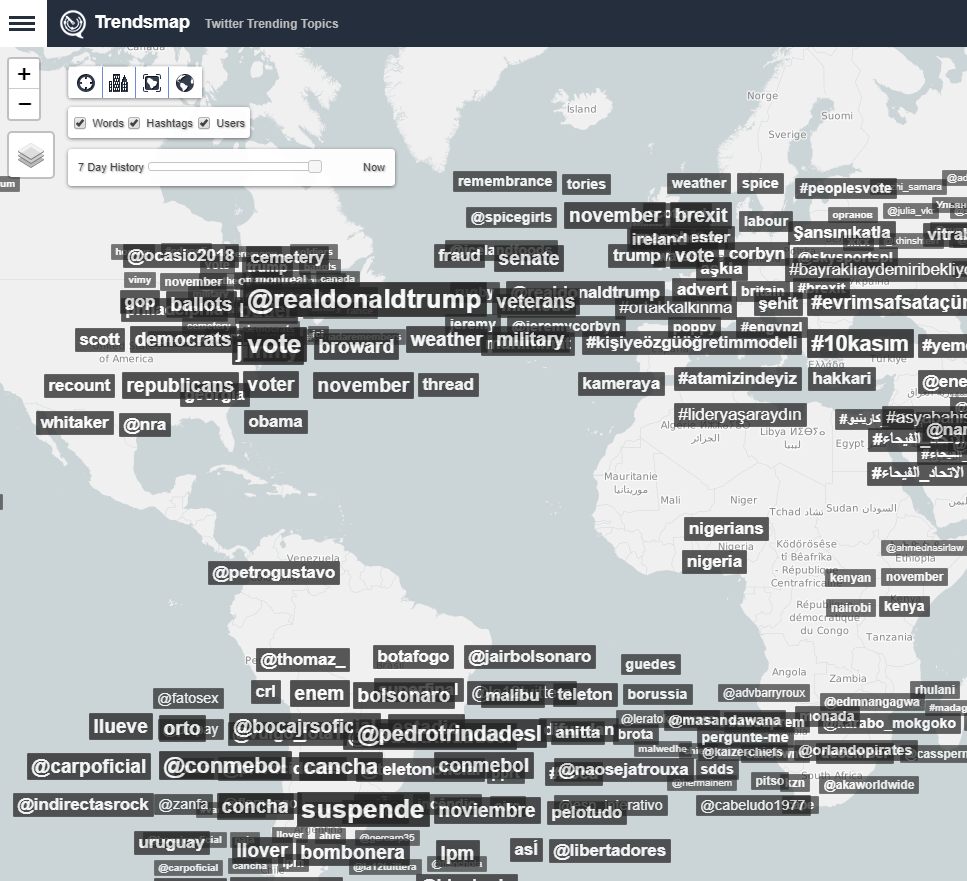
\includegraphics[scale=0.383]{trendsmap}
\caption{TrendsMap Interface}
\end{figure}
\\
The main difference between our system and the available web mashups however is that we are developing a framework that does not revolve around a specific topic. Instead, the data integration procedures and the context-awareness applications are generalized and made adaptable to numerous situations.\\\\
Integrating data incoming from heterogenous sources has been a topic of interest for many years now. The work proposed in \cite{braga} focuses on multi-domain queries, i.e. queries that make use of two or more heterogeneous resources available on the web. The authors try to create a formal abstraction of the query, and then map the query to multiple ``query plans''. A query plan represents a possible execution schedule for these queries, either sequentially or in parallel, depending on which combination has the best performance.\\\\
Francese et al.\cite{dynamicapp} proposed an interesting approach that allows users to use dynamically design their own applications on their smartphones, in a process that integrates the functionalities of their devices with Internet services. Although their approach grants great freedom to users to decide and design how to access these resources, it does not focus on the context of the users, and does not personalize the user experience based on the conditions of each individual user.\\\\
Another service dubbed ``MyService'' was created by Lee and Joo\cite{myservice}; their platform allows experienced designers to specify rules that define the context. These rules determine which services are selected, and dynamic code generation takes care of invoking these services at runtime. However, this system only considers location as the main factor that defines the context. Our definition of context is much broader, and include many factors, one of which is location. Moreover, the selection of the services that the system should query is done by the system itself in our case, and the users do not need to decide which service to query. Service selection is done by identifying the needed resources, and querying the services that would best fulfill these needs automatically.\\\\
Casillo et al.\cite{casillo} developed a context-aware mobile application that aims to help tourists in Salerno plan their trip and locate places of interest. In their approach, the authors used a context dimension tree to specify various parameters of a user's context, and their definition of context is very close to ours. The results of their work was very promising; one hundred users installed and used the application, and afterwards filled a survey to describe their experience. In most cases, user satsifaction rate was above 75\%, and they generally agreed that the application's interpretation of their context is accurate. This is encouraging for us because it implies that using a context dimension tree to describe a user's context is a valid approach. An additional feature in our system is the dynamic inclusion of web services: the services that can be queries are not fixed, and new services can be always added to provide more -and more accurate- results.\\\\
To wrap up, there are many projects that have tried to approach data integration and mashups from different angles. Many of the presented solutions are well structured and do their intended work efficiently. However, they are still missing one or more of the key elements we are focusing on in our system, whether it is a clear and comprehensive definition of ``context'', an efficient representation of this context (both in terms of abstract design and practical implementation), or a valid generalization of the web service integration operations.